\section{Spin injection}\label{sec:spin-injection}

\subsection{Introduction}

In this section we discuss how light can be used to manipulate spins inside a solid-state material.

We start by considering a semiconductor and the energy dispersion around the center of the Brillouin zone, $\Gamma \equiv (0,0,0)$, where the band structure is typically divided into two main parts:
\begin{itemize}
    \item \textbf{Conduction band}: an $s$-type antibonding band.
    \item \textbf{Valence band}: a $p$-type bonding band, which is split into three sub-bands, namely heavy holes (HH), light holes (LH), and the split--off (SO) band, due to spin--orbit coupling.
\end{itemize}
The HH and LH bands are degenerate at the Brillouin zone center, while the SO band is separated by the spin--orbit interaction.

Let us assume the following conditions:
\begin{enumerate}
    \item the optical transitions are dipole allowed;
    \item a four-band model is sufficient near $k \simeq 0$;
    \item subsidiary minima at $k \neq 0$ can be neglected.
\end{enumerate}

\question{From the band structure alone, can we conclude that the material is magnetic?}{The answer is no, because in the absence of an external magnetic field the electronic states are spin degenerate. In particular, the conduction band states are doubly degenerate, corresponding to spin-up $(m_s=+1/2)$ and spin-down $(m_s=-1/2)$.}

\subsection{Optical spin orientation}

\subsubsection{Light can carry angular momentum}
A net spin population can be created by using circularly polarized light. This mechanism is widely exploited in quantum technologies, such as spin-photon interfaces, and in spintronics applications such as spin-LEDs and spin lasers.

\calloutinfo{Circularly polarized light carries angular momentum along the propagation direction. In particular, right- and left-handed circular polarizations, usually denoted by $\sigma^+$ and $\sigma^-$, correspond to angular momentum $\pm \hbar$, respectively, depending on the handedness convention.}

A circularly polarized electric field can be viewed as the superposition of two orthogonal components, $E_x$ and $E_y$, oscillating with a relative phase shift of $\lambda/4$.
\begin{figure}[H]       
    \centering            
    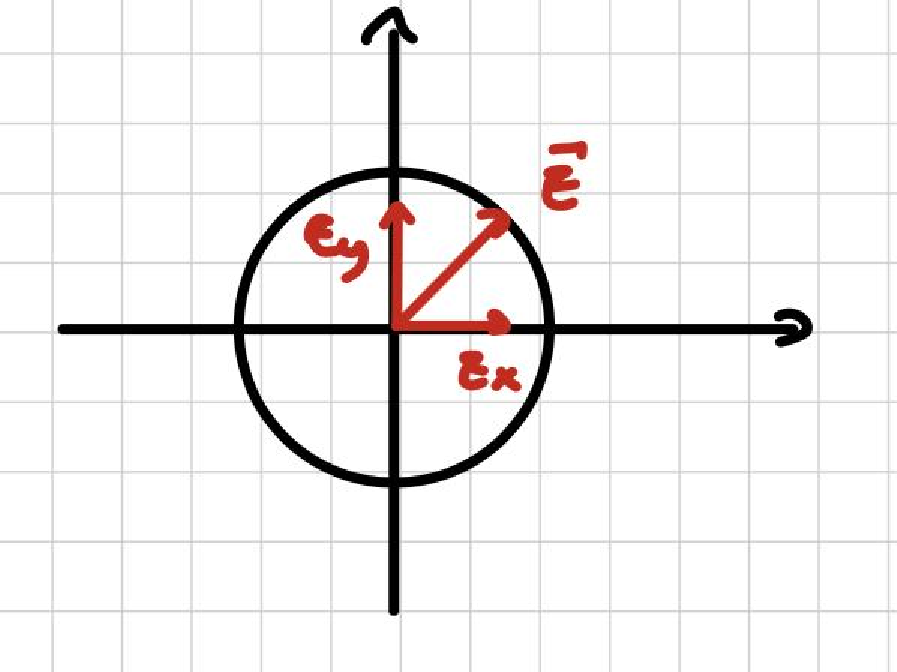
\includegraphics[width=0.8\textwidth]{images_in_pdf/3-/Grafico_6.pdf} 
\end{figure}

When a single electron absorbs circularly polarized light, the response is an acceleration caused by the rotating electric field (circular orbits). The connection with angular momentum can be understood by comparing the power delivered by the electromagnetic field with the power associated with a torque:
\[
P_1 = \odv{\varepsilon}{t}, \qquad P_2 = \tau \omega,
\]

where $\tau$ is the torque and $\omega$ the angular frequency. Since torque is the rate of change of angular momentum on average, one has
\[
P_1 = P_2 \implies \odv{\varepsilon}{t} = \omega \odv{L}{t},
\]

so that the absorbed angular momentum per quantum of energy is
\[
\varepsilon = \hbar \omega \implies L = \frac{\varepsilon}{\omega} = \hbar.
\]

Therefore, each circularly polarized photon carries angular momentum $\pm \hbar$, with the sign determined by the helicity.
\begin{figure}[H]       
    \centering            
    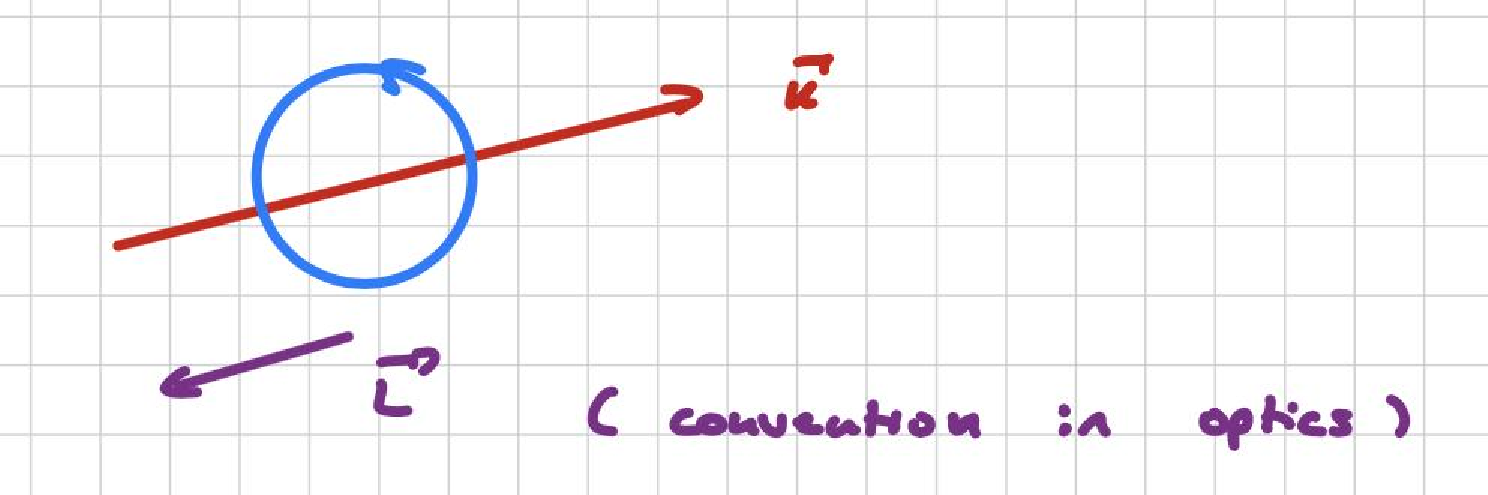
\includegraphics[width=0.8\textwidth]{images_in_pdf/3-/Grafico_7.pdf} 
\end{figure}

For this reason, we distinguish two \textbf{helicity states} of circularly polarized light:
\begin{itemize}
    \item $\ket{L}$ transfers angular momentum to the target as if the photon spin were aligned with the propagation direction;
    \item $\ket{R}$ reverses the handedness and transfers angular momentum with opposite sign.
\end{itemize}

\subsubsection{Transition rates}
In the semiconductor:
\begin{itemize}
    \item The conduction band is $s$-like, so $\ell=0$ and the states are characterized by $j=\ell+s = 1/2$.
    
    \item The valence band is $p$-like and, after including spin-orbit coupling, is described by the total angular momentum $j$, with $\ell-s \leq j \leq |\ell+s| \implies j = \frac{1}{2},\frac{3}{2}$: the states split into $j=3/2$ (HH and LH) and $j=1/2$ (SO).
\end{itemize} 
The corresponding magnetic quantum number satisfies $-j \leq m_j \leq +j$ along the quantization axis, which is taken to be the propagation direction.
\begin{figure}[H]       
    \centering            
    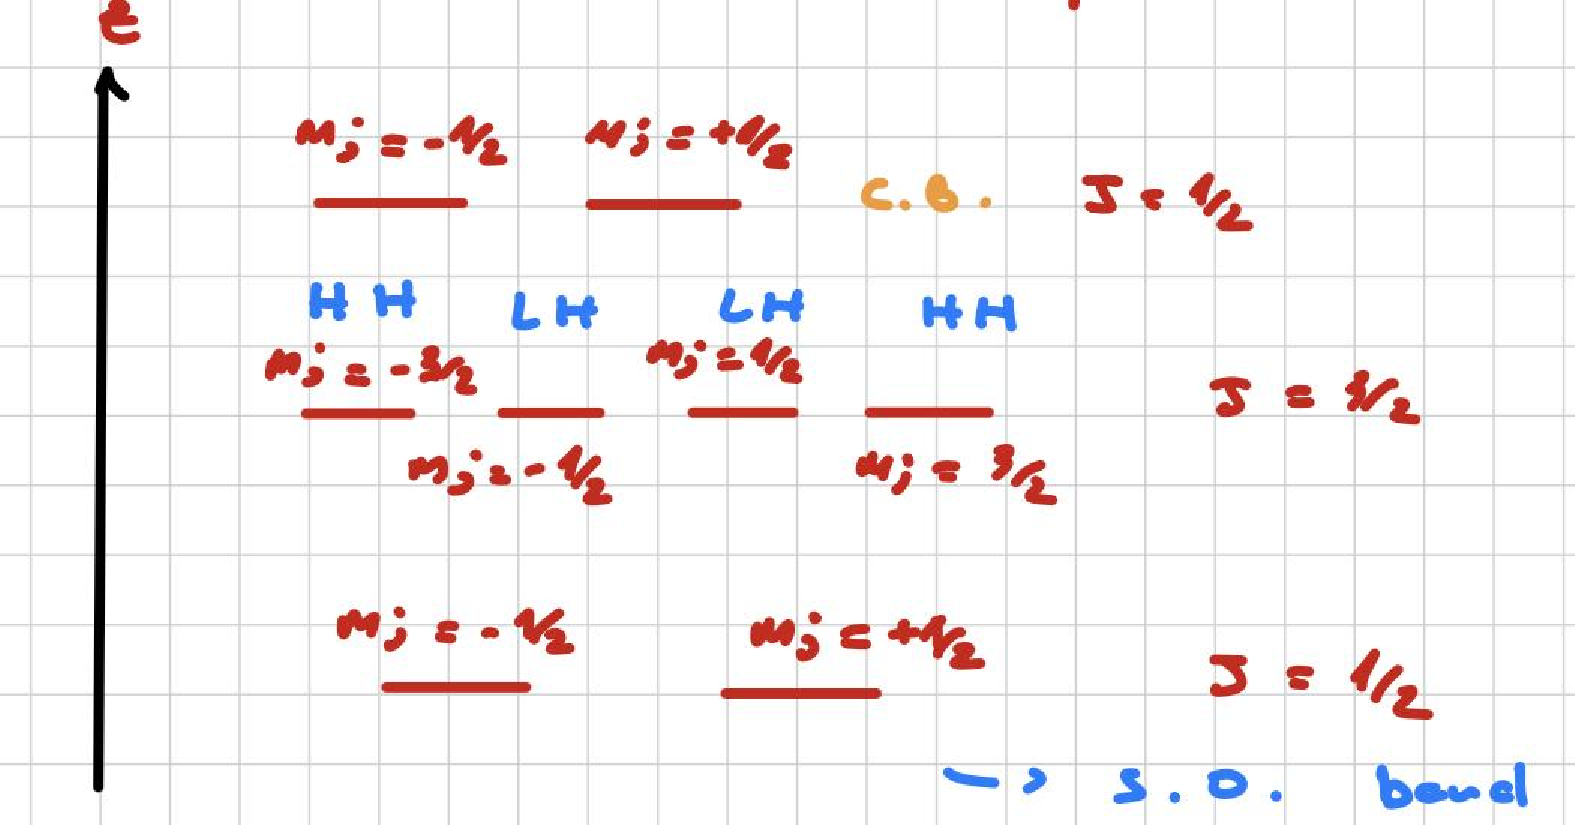
\includegraphics[width=0.8\textwidth]{images_in_pdf/3-/Grafico_8.pdf} 
\end{figure}

To compute the transition rate, we evaluate the matrix element
\begin{equation}\label{eqn:3-radiative-transition-matrix-element}
M = \bra{\psi_f}\hat{H}_{\text{int}}\ket{\psi_i}
\end{equation}

where, in the electric dipole approximation,
\[
\hat{H}_{\text{int}} = -\vec{d}\cdot \vec{E}_0,
\qquad
\vec{d} = -e\vec{r},
\]

with $\vec{r}=\hat{x}+\hat{y}+\hat{z}$ being the position vector of the electron and $\vec{E}_0$ the electric field amplitude.

The wave function can be factorized into a radial part and an angular part,
\[
\psi_{n,\ell,m}(r,\theta,\phi) = R_{n,\ell}(r)\,Y_{\ell,m}(\theta,\phi),
\]

so that the matrix element is obtained by integrating over the full spatial coordinates.
\[
M = \int_0^{+\infty} \d{r} \cdot \int_0^{\pi} \d\theta \cdot \int_0^{2\pi} \d\phi \cdot \psi_f^*\cdot  \hat{H} \cdot \psi_i\cdot r^2 \sin^2(\theta)
\]

The dot product between the dipole operator and the electric field is proportional to:

\begin{equation}
\vec{e}_{\sigma^{\pm}} = \frac{1}{\sqrt{2}}\cdot (\hat{x} \pm i\hat{y})
\implies 
\vec{e}_{\sigma^{\pm}} \cdot \vec{r} =
\frac{1}{\sqrt{2}}\cdot (x \pm i y)
\end{equation}

Then, in polar coordinates:
\begin{equation}
\begin{cases}
    x=r\cos\phi\\[0.5ex]
    y=r\sin\phi
\end{cases}
\implies
x \pm i y = r(\cos\phi \pm i \sin\phi) 
\equiv r e^{\pm i\phi}
\end{equation}

The angular part of the matrix element is therefore proportional to:
\[
M_{\sigma^{\pm}} \propto \int_0^{2\pi} d\phi\cdot  Y_{\ell',m'}^*(\theta,\phi) \cdot e^{\pm i \phi} \cdot Y_{\ell,m}(\theta,\phi) \propto \int_0^{2\pi} d\phi\cdot  e^{-im'\phi} \cdot e^{\pm i \phi} \cdot e^{im\phi} \ne 0
\]

which is nonzero only if the selection rule
\begin{equation}\label{eqn:3-dipole-selection-rule}
\Delta m_\ell = \pm 1
\end{equation}

is satisfied. Since spin cannot change under electric dipole transitions, the condition on $m_\ell$ results in one on $m_j$; circularly polarized light couples only to specific transitions:
\begin{itemize}
    \item $m_j' = m_j + 1, \Delta m_j = +1 \iff \sigma^+$ transition;
    
    \item $m_j' = m_j - 1, \Delta m_j = -1 \iff \sigma^-$ transition.
\end{itemize}
For this reason, only a restricted set of optical transitions is allowed.

\begin{figure}[H]       
    \centering            
    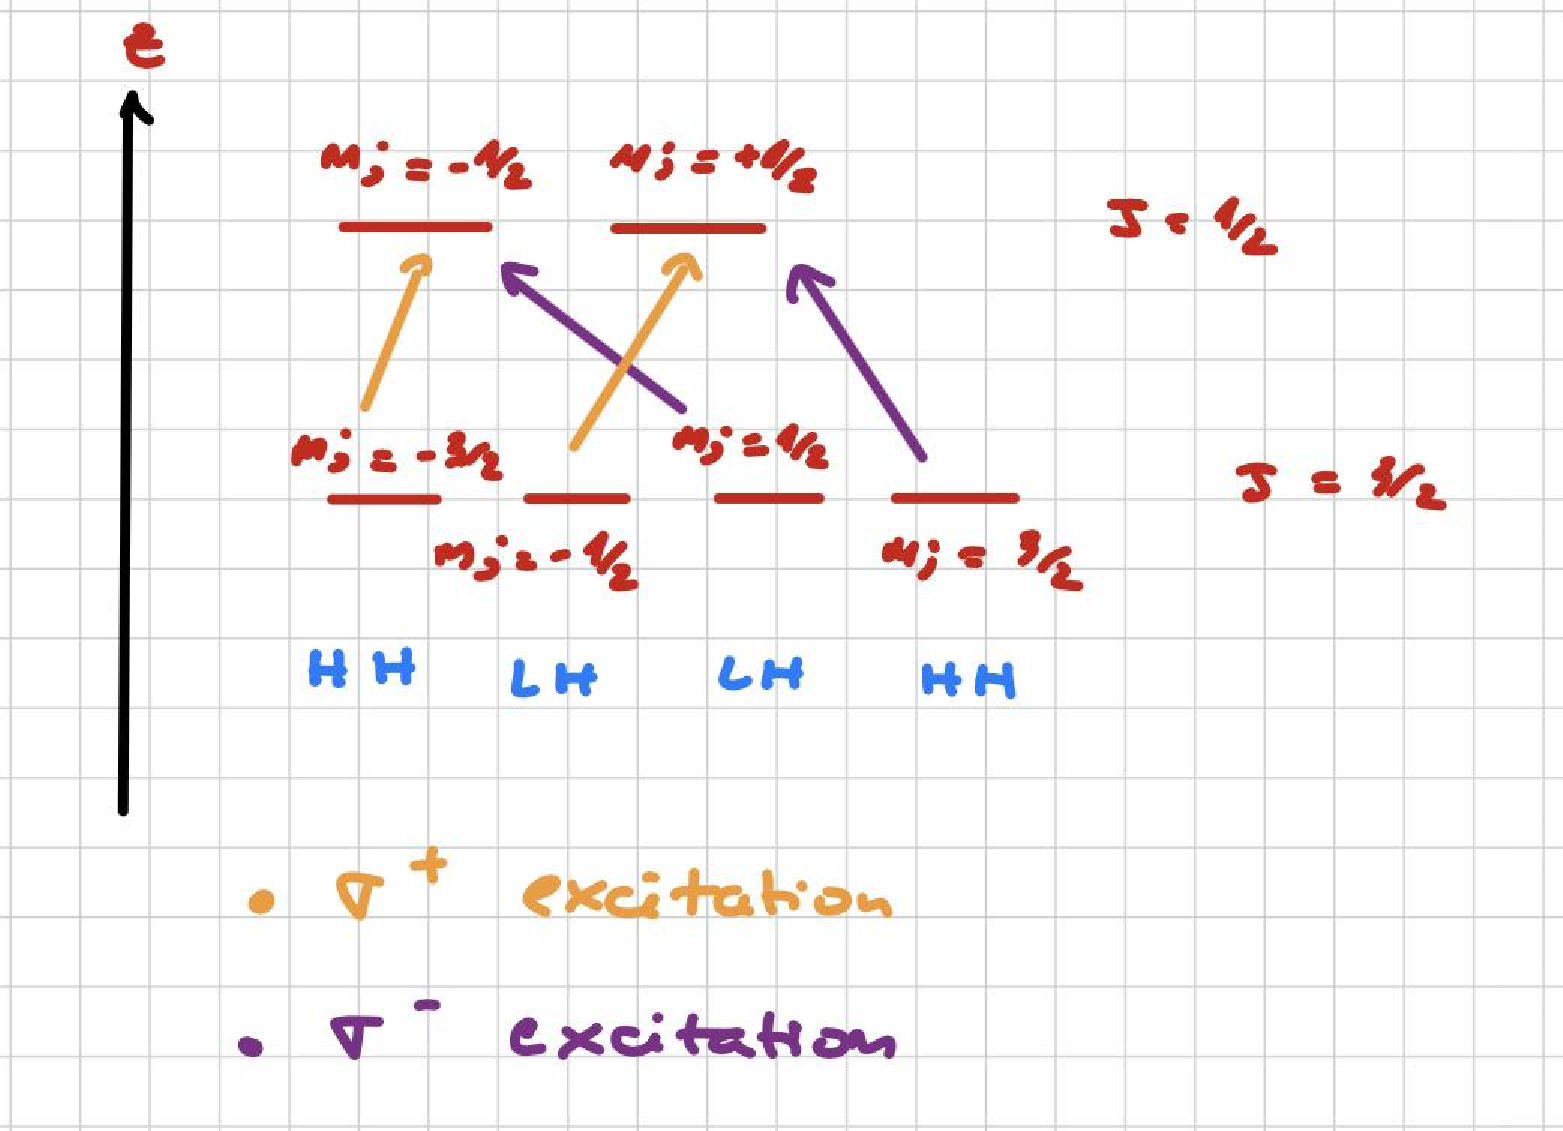
\includegraphics[width=0.8\textwidth]{images_in_pdf/3-/Grafico_9.pdf} 
\end{figure}

Using Fermi's golden rule, stating the transition rate is proportional to $|M|^2$, can be shown that:
\[
|M_{HH}|^2 = 3|M_{LH}|^2.
\]

This imbalance means that \hl{transitions involving heavy--hole states are favored over light--hole states}.
\begin{figure}[H]       
    \centering            
    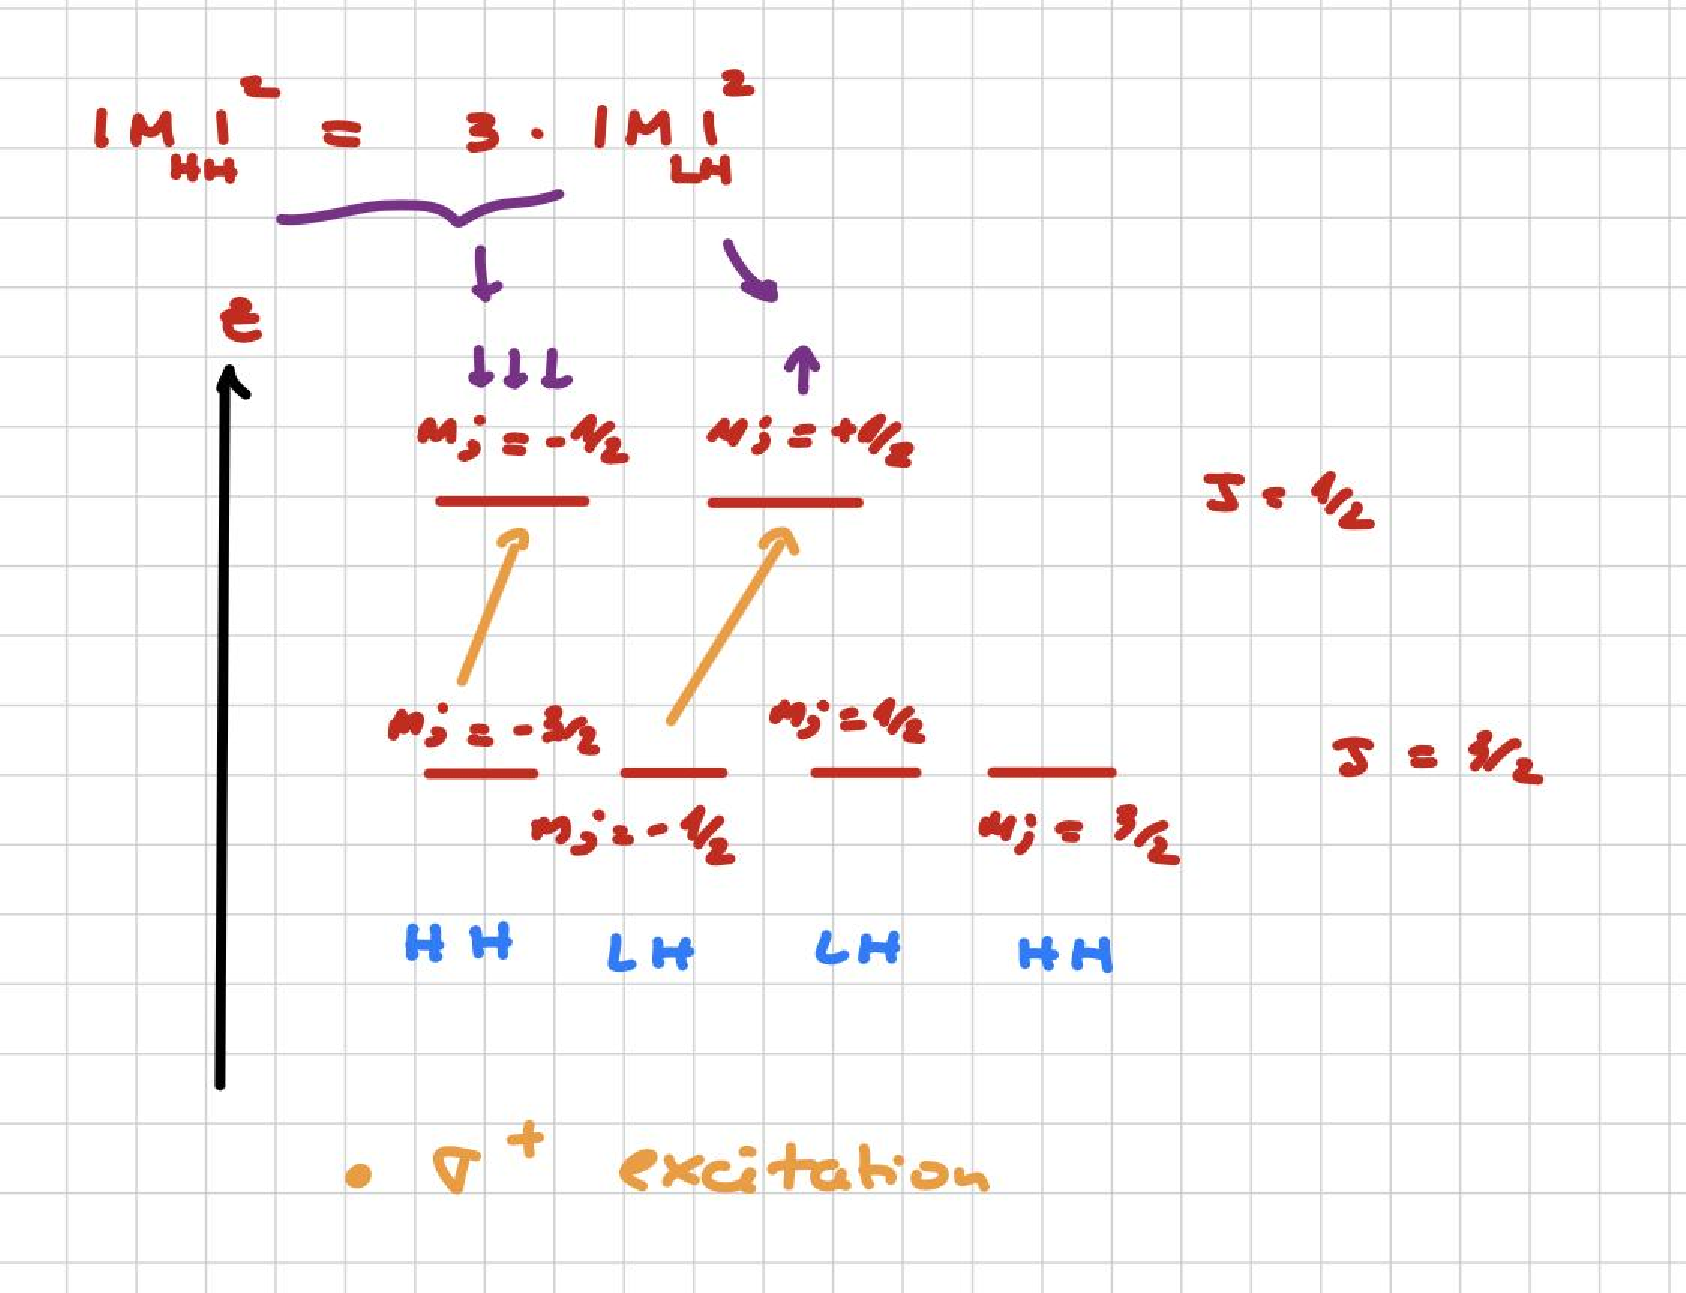
\includegraphics[width=0.8\textwidth]{images_in_pdf/3-/Grafico_10.pdf} 
\end{figure}

As a consequence, the excited carrier population becomes spin polarized. 
In the simplest bulk model, the resulting electron spin polarization is
\begin{equation}\label{eqn:3-spin-polarization}
P_s = \frac{N(+1/2)-N(-1/2)}{N(+1/2)+N(-1/2)} = 
\frac{1-3}{1+3}= -50\%
\end{equation}

\calloutinfo{The same idea applies to holes, but their spin polarization is usually much less robust because spin--orbit coupling in the valence band causing rapid spin relaxation. For electrons in the $s$-type ($\ell=0$) conduction band, this effect is much weaker, since the orbital angular momentum is approximately zero and therefore $\vec{L}\cdot \vec{S}$ is small.}

If the system is excited with $\sigma^+$ light and the split--off states ($\ell=1, m_\ell=0$) are also included, one finds that
\[
|M_{SO}|^2 = 2|M_{LH}|^2.
\]

\begin{figure}[H]       
    \centering            
    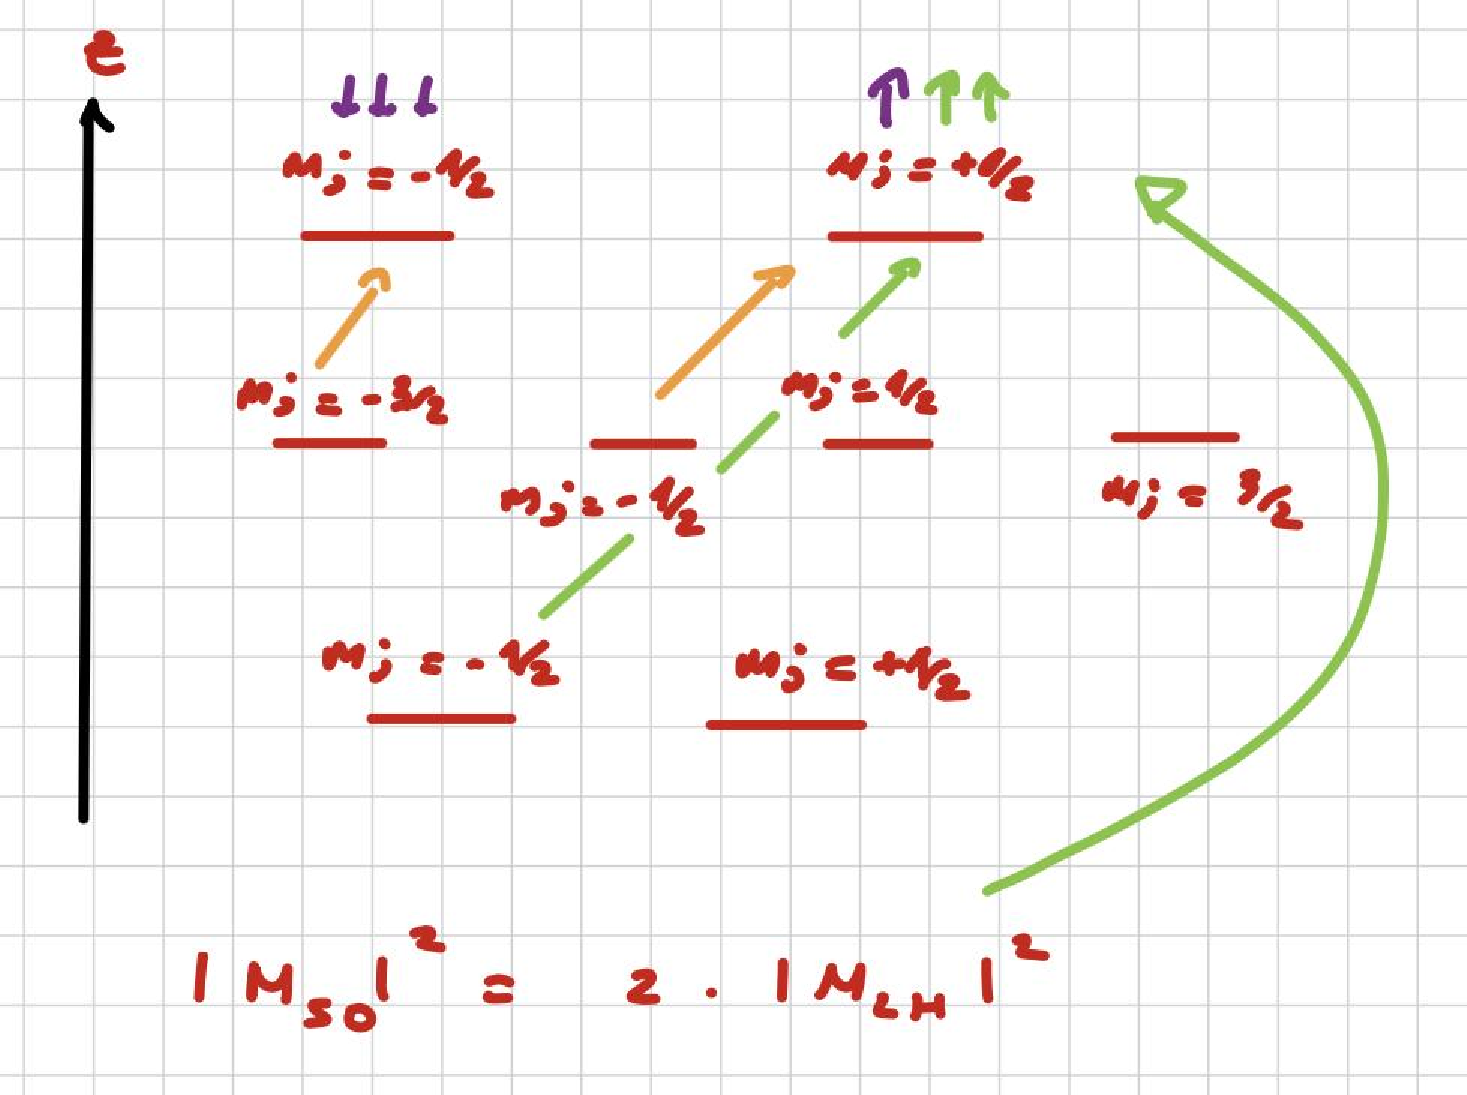
\includegraphics[width=0.8\textwidth]{images_in_pdf/3-/Grafico_11.pdf} 
\end{figure}

As a result, the electron spin polarization exhibits a clear spectral dependence. At the bandgap threshold, where the split-off band is not yet accessible, the polarization reaches its peak value of 50\%. Beyond this onset, the net polarization becomes a function of the photon energy:
\[
P_s = P_s(E=\hbar\omega).
\]
\begin{figure}[H]       
    \centering            
    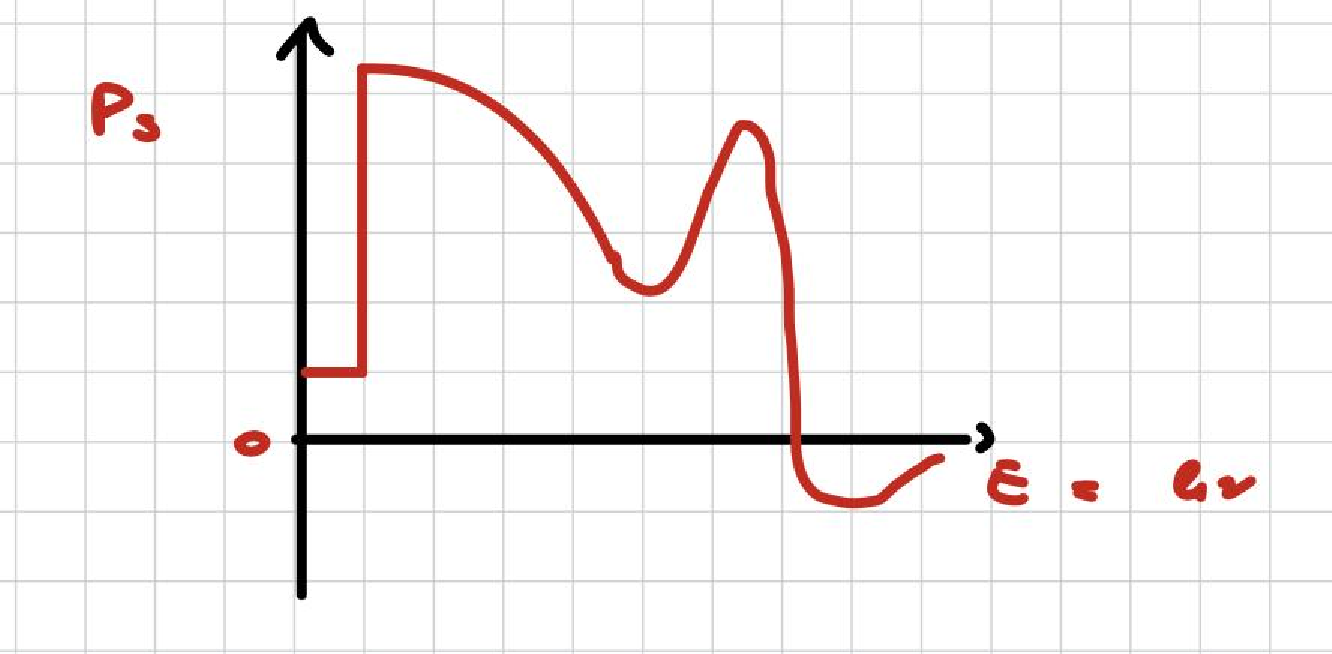
\includegraphics[width=0.8\textwidth]{images_in_pdf/3-/Grafico_12.pdf} 
\end{figure}

\calloutwarn{The split--off band becomes relevant at higher photon energies, where it drives the polarization toward smaller and even negative values. This behavior is related to the band curvature and to the density of states, which determine how many transitions contribute at each energy. Moreover, away from the center of the Brillouin zone, the HH and LH bands are no longer degenerate and their character becomes mixed, making the problem more complicated.}

\subsection{Experimental determination of spin polarization}

While analytically modeling this $P_s(E)$ behavior away from the Brillouin zone center is highly complex due to these band-mixing effects, we can experimentally determine the spin polarization by exploiting optical techniques. Since the selection rules governing absorption must also dictate the radiative recombination of spin-polarized carriers, we can rely on \textbf{circularly polarized photoluminescence} (PL) as a direct probe. By measuring the luminescence polarization, and assuming that the same transition rules remain valid for recombination:
\begin{figure}[H]       
    \centering            
    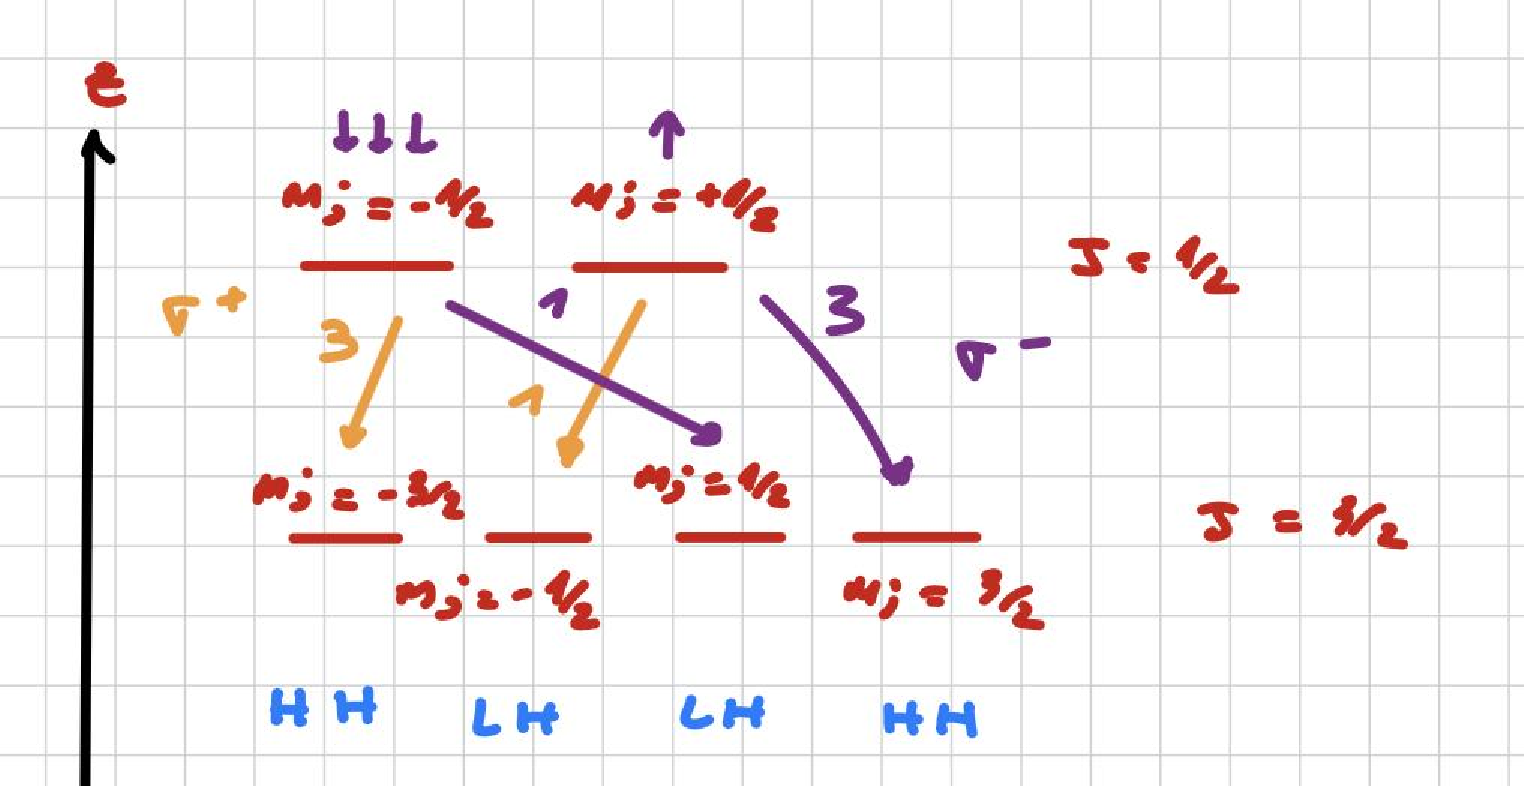
\includegraphics[width=0.8\textwidth]{images_in_pdf/3-/Grafico_13.pdf} 
\end{figure}

\[
\rho_c = \frac{I^+ - I^-}{I^+ + I^-}
= \frac{(1\cdot n_{\uparrow} + 3\cdot n_{\downarrow}) - (3\cdot n_{\uparrow} + 1\cdot n_{\downarrow})}
{(1\cdot n_{\uparrow} + 3\cdot n_{\downarrow}) + (3\cdot n_{\uparrow} + 1\cdot n_{\downarrow})}
= 25\% = -\frac{P_s}{2},
\]

where $I^\pm$ denotes the intensity of the luminescence component with helicity $\sigma^\pm$.

This shows that the maximum observable polarization in this simplified bulk picture is $25\%$, although experimentally the measured value is usually smaller.
\begin{figure}[H]       
    \centering            
    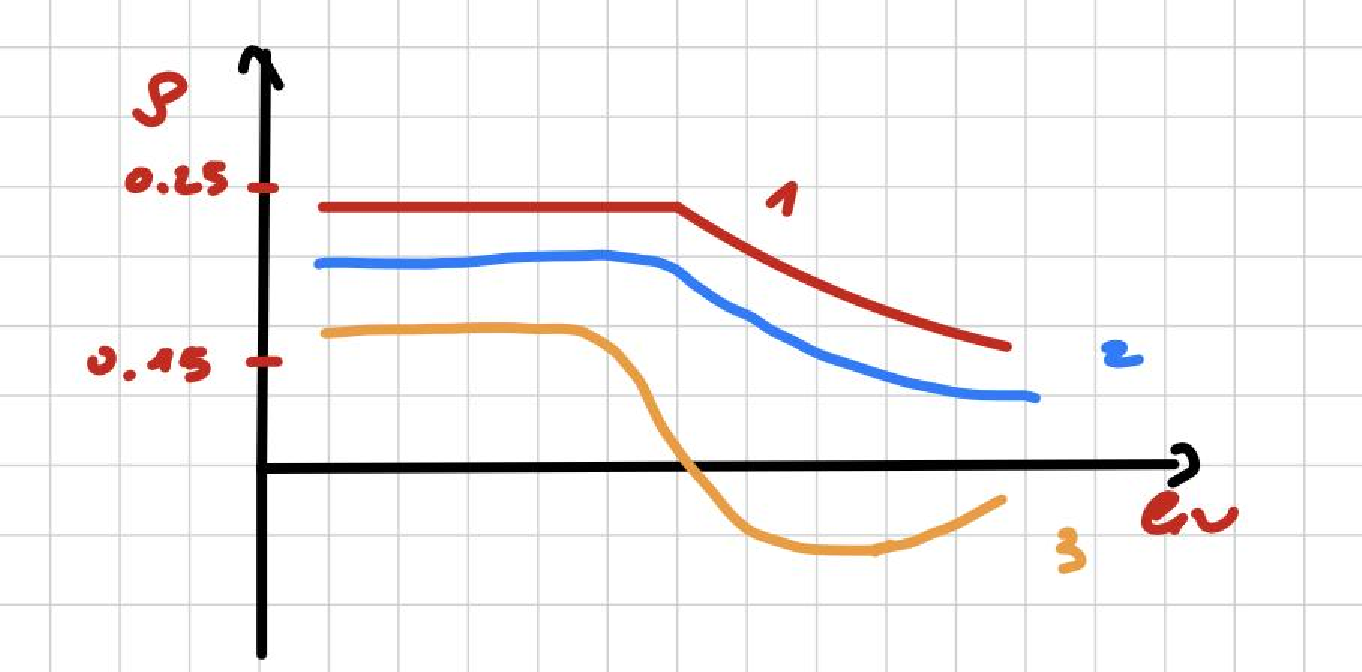
\includegraphics[width=0.8\textwidth]{images_in_pdf/3-/Grafico_14.pdf} 
\end{figure}

The reduction is caused by spin-relaxation mechanisms acting between optical excitation and recombination:
\[
\rho_c = \frac{\rho_0}{1+\tau/\tau_s},
\]

where $\rho_0$ is the polarization in the absence of spin relaxation, $\tau$ is the carrier lifetime, and $\tau_s$ is the spin-relaxation time. Thus,
\begin{itemize}
    \item if $\tau \gg \tau_s$, then $\rho_c \to 0$;
    \item if $\tau \ll \tau_s$, then $\rho_c \to \rho_0$.
\end{itemize}
The main spin-relaxation mechanisms are:
\begin{enumerate}
    \item \textbf{Dyakonov-Perel mechanism:} it occurs in crystals lacking inversion symmetry. Spin degeneracy is lifted by spin-orbit coupling, which acts as an effective magnetic field $\vec{B}_{\mathrm{eff}}$. The direction of this effective field changes randomly during scattering events, leading to spin depolarization through a sequence of random precessions. This mechanism does not occur in centrosymmetric materials such as Si or Ge.
    \item \textbf{Elliott-Yafet mechanism:} it is important in narrow-gap semiconductors. Strong spin-orbit coupling mixes spin-up and spin-down components in the wave functions, so scattering events can cause spin flips and reduce the polarization.
    \item \textbf{Bir-Aharonov-Picus mechanism:} it originates from exchange interaction between electrons and holes, which can induce electron spin flips.
\end{enumerate}

\subsection{Spin injection in low-dimensional structures}

\question{How can we improve the spin polarization?}{%
    The main limitation in the bulk case is that optical excitation generally involves both HH and LH states, which reduces the achievable polarization. A way to enhance the spin selectivity is to remove the HH-LH degeneracy using low-dimensional structures.
}

A particularly useful example is a quantum well made of alternating \ce{GaAs} and \ce{AlGaAs} layers, where the \ce{GaAs} thickness $t$ is chosen such that
\[
t \lesssim \lambda_{\mathrm{dB}},
\]
with $\lambda_{\mathrm{dB}}$ being the de Broglie wavelength of the carriers.
\begin{figure}[H]       
    \centering            
    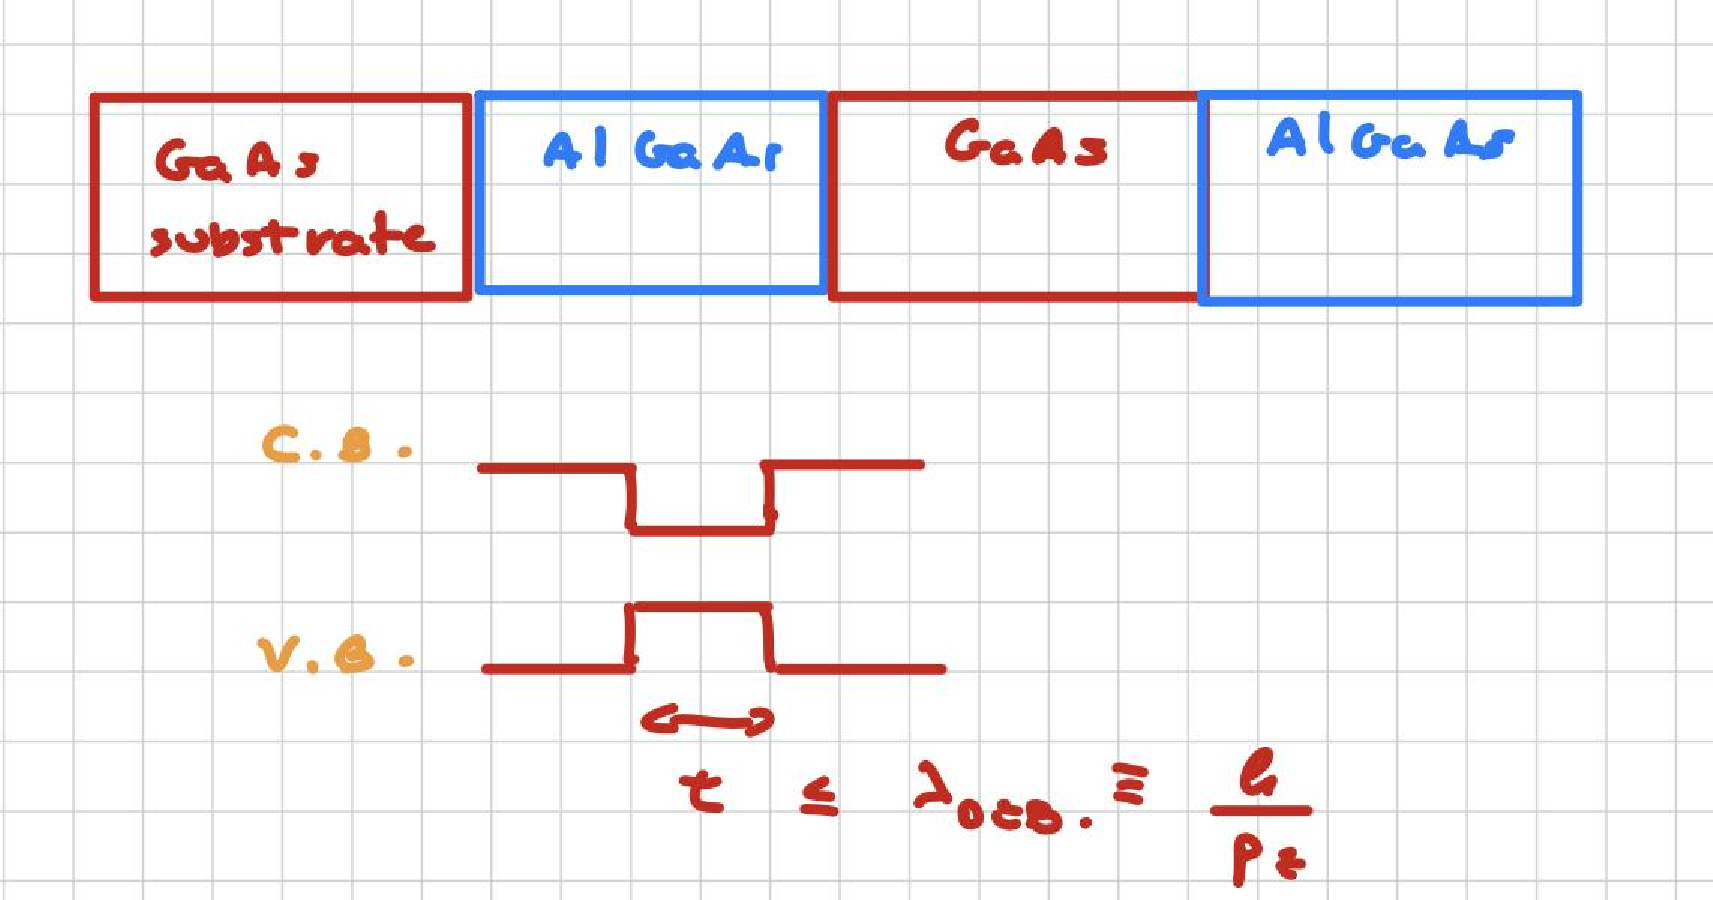
\includegraphics[width=0.8\textwidth]{images_in_pdf/3-/Grafico_15.pdf} 
\end{figure}

In this regime, quantum confinement becomes important and the system behaves approximately like a particle in a box, with discrete energy levels:
\[
E_n = \frac{\hbar^2}{2m^*}\left(\frac{n\pi}{L}\right)^2.
\]

\calloutinfo{Since the confinement energy depends on the effective mass $m^*$, it is different for HH and LH states. As a result, the two bands are split, hence the two transitions require different energies. If the system is excited with circularly polarized light in this energy window:
\[
E_g + E_{e_1} + E_{HH_1} \leq \hbar\omega \leq E_g + E_{e_1} + E_{LH_1},
\]
one can in principle obtain $100\%$ electron spin polarization.}

Here:
\begin{itemize}
    \item $E_g$ is the band gap;
    \item $E_{e_1}$ is the confinement energy of the first electron sub-band;
    \item $E_{HH_1}$ is the first confinement energy of the HH sub-band;
    \item $E_{LH_1}$ is the first confinement energy of the LH sub-band.
\end{itemize}
\begin{figure}[H]       
    \centering            
    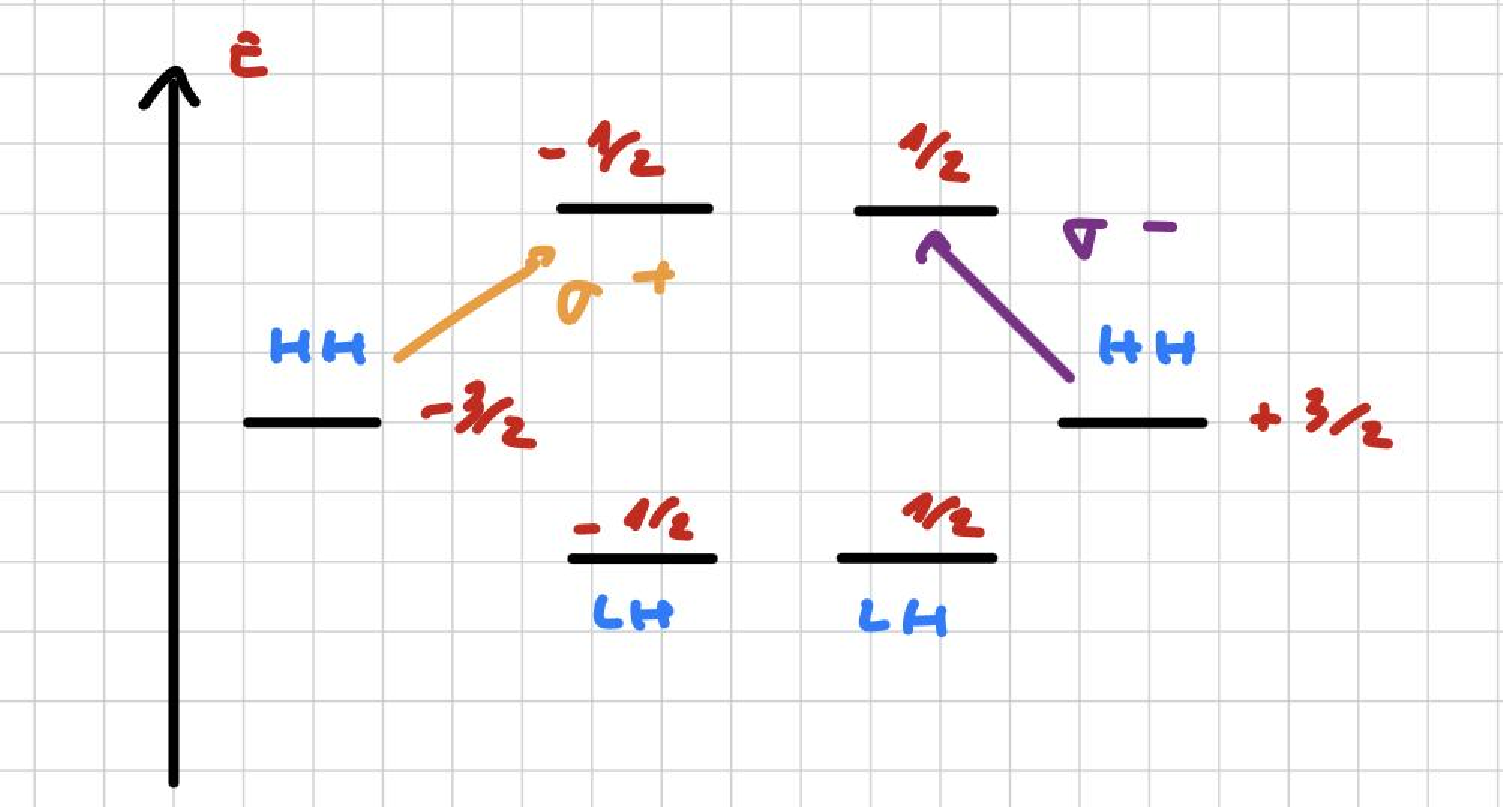
\includegraphics[width=0.8\textwidth]{images_in_pdf/3-/Grafico_16.pdf} 
\end{figure}

In this way one can reach an electron polarization degree
\[
P_c = \pm 100\%,
\]

where the sign depends on the helicity $\sigma^\pm$.

\hl{The key point is that the spin orientation is determined by the helicity of the light.}

Notice that the splitting of the valence sub-bands suppresses HH-LH mixing and also reduces spin relaxation of the holes compared with the bulk case.

\subsection{Spin quantum beat}\label{subsec:3-spin-quantum-beat}

Suppose we send circularly polarized $\sigma^+$ light pulses propagating along the $z$-axis onto a \ce{GaAs} quantum well and then apply an external magnetic field along the $x$-axis, $\vec{B}_{\mathrm{ext}} = B_{\mathrm{ext}} \hat{x}$. 

\calloutinfo{In this situation, the photoexcited spins undergo Larmor precession, so that the expectation value of the spin component along $z$, $\langle \hat{S}_z \rangle$, oscillates in time between positive and negative values. This effect is known as a \textbf{spin quantum beat}.}

\begin{figure}[H]\label{fig:3-spin-quantum-beat}
    \centering            
    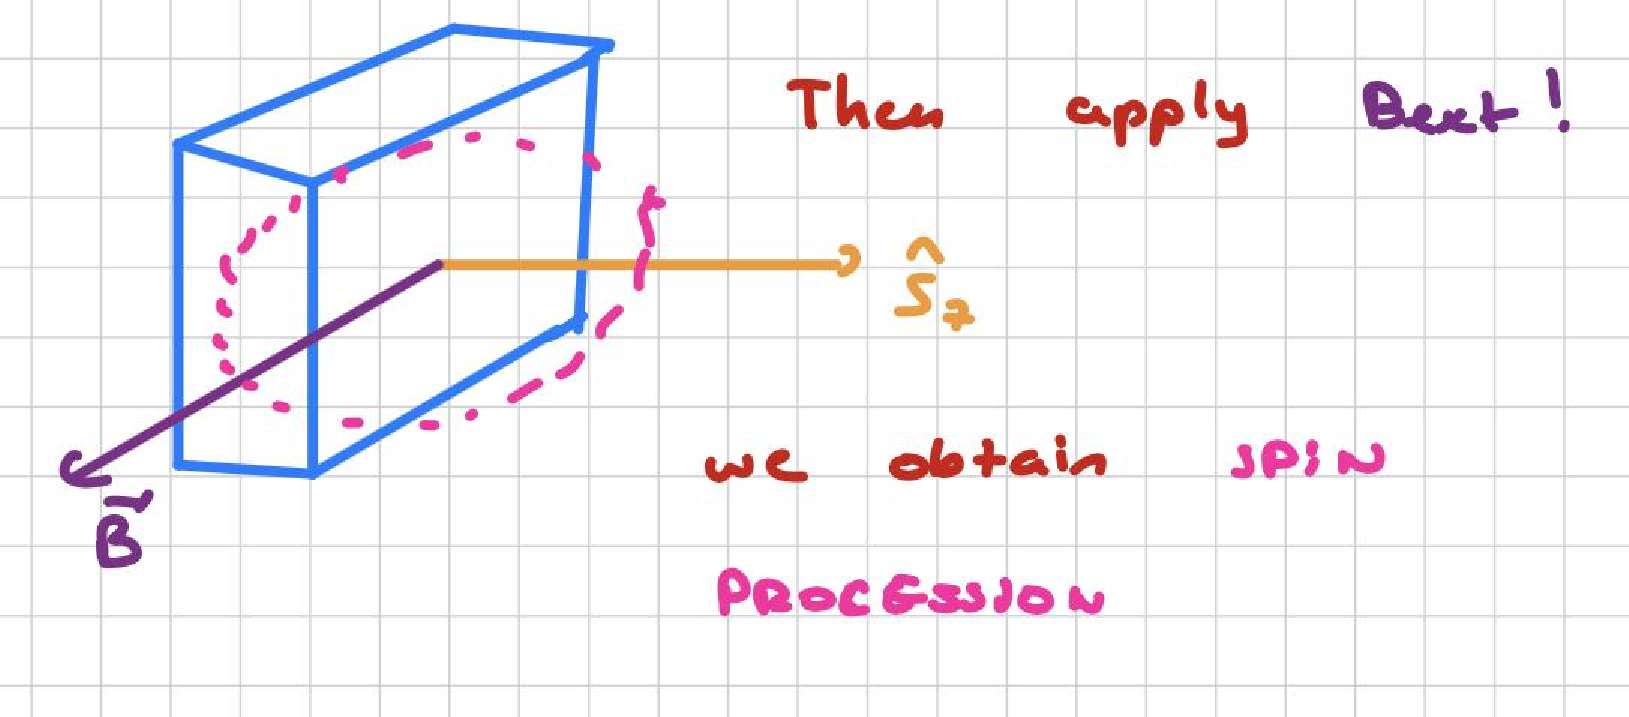
\includegraphics[width=0.8\textwidth]{images_in_pdf/3-/Grafico_17.pdf} 
\end{figure}

\subsubsection{Zeeman hamiltonian}

The Zeeman hamiltonian describes the interaction between the spin and the external magnetic field:
\begin{equation}\label{eqn:3-zeeman-hamiltonian}
\hat{H}_Z = -\vec{\mu}\cdot \vec{B}_{\mathrm{ext}} =
-g \mu_B \hat{\vec{S}}\cdot \vec{B}_{\mathrm{ext}},
\end{equation}

where $\vec{\mu}$ is the magnetic moment, $g$ is the carrier $g$-factor, $\mu_B$ is the Bohr magneton, and $\hat{\vec{S}}$ is the spin operator. In our case, since $\vec{B}_{\mathrm{ext}}$ is along $\hat{x}$,
\begin{equation}\label{eqn:3-zeeman-hamiltonian-2}
\hat{H}_Z =
-g \mu_B \hat{S}_x B_{\mathrm{ext}} =
-g \mu_B \frac{\hbar}{2} \hat{\sigma}_x B_{\mathrm{ext}}
\end{equation}

where we used the relation $\hat{S}_x = \frac{\hbar}{2} \hat{\sigma}_x$ between the spin operator and the Pauli matrix. Defining the \textbf{Larmor frequency} as $\omega_L = \frac{|g|\mu_B B_{\mathrm{ext}}}{\hbar}$, the hamiltonian becomes:
\begin{equation}\label{eqn:3-zeeman-hamiltonian-3}
    \hat{H}_Z = -\frac{1}{2} \hbar \omega_L \hat{\sigma}_x
\end{equation}

therefore its eigenstates are exactly the spin ones $\ket{\uparrow_x}$ and $\ket{\downarrow_x}$ with eigenvalues $\pm \frac{1}{2}\hbar \omega_L$.

\subsubsection{Spin dynamics}
As seen in the spin--injection process, the $\sigma^+$ pulse creates a neat population of spin--up electrons along the $z$-axis. Such state, $\ket{\uparrow_z}$, is a superposition of the two spin eigenstates along the $x$-axis, $\ket{\uparrow_x}$ and $\ket{\downarrow_x}$:
\begin{equation}\label{eqn:3-spin-superposition}
    \ket{\uparrow_z} = \frac{1}{\sqrt{2}}\left(\ket{\uparrow_x} + \ket{\downarrow_x}\right)
\end{equation}

Written like this, the time evolution of $\ket{\uparrow_z}$ under the Zeeman hamiltonian (Eqn.~\ref{eqn:3-zeeman-hamiltonian-3}) is straightforward to compute:
\begin{equation}\label{eqn:3-spin-superposition-time-evolution}
\ket{\uparrow_z(t)} = 
\frac{1}{\sqrt{2}}\left(\ket{\uparrow_x}e^{i\omega_L t/2} +
\ket{\downarrow_x}e^{-i\omega_L t/2}\right)
\end{equation} 

where the time--evolution operator $U(t) = e^{-i\hat{H}_Z t/\hbar}$ was used. Then, we can express the $x$--basis states in terms of the $z$--basis states, and perform a simple regroup of the terms:
\begin{equation}\label{eqn:3-x-basis-in-z-basis}
\begin{split}
\ket{\uparrow_z(t)} &=
\frac{1}{2}
\left[
\left(\ket{\uparrow_z}+\ket{\downarrow_z}\right)e^{i\omega_L t/2} +
\left(\ket{\uparrow_z}-\ket{\downarrow_z}\right)e^{-i\omega_L t/2}
\right]=\\[0.5ex]
&=\frac{1}{2}
\left[
\ket{\uparrow_z}\left(e^{i\omega_L t/2} + e^{-i\omega_L t/2}\right) +
\ket{\downarrow_z}\left(e^{i\omega_L t/2} - e^{-i\omega_L t/2}\right)
\right]
\end{split}
\end{equation}

here, we apply the Euler's formula:
\begin{equation}\label{eqn:3-euler-formula}
\begin{cases}
\cos\alpha = \frac{e^{i\alpha} + e^{-i\alpha}}{2}\\[0.5ex]
\sin\alpha = \frac{e^{i\alpha} - e^{-i\alpha}}{2i}
\end{cases}
\end{equation}

and we finally obtain:
\begin{equation}\label{eqn:3-spin-superposition-time-evolution-final}
\ket{\uparrow_z(t)} =
\ket{\uparrow_x}\cos\left(\frac{\omega_L t}{2}\right) + i\ket{\downarrow_x}\sin\left(\frac{\omega_L t}{2}\right)
\end{equation}

\calloutwarn{This means that the system oscillates coherently between spin--up and spin--down components.}


% questa immagine viene BOCCIATA! non ha senso
\begin{comment}
\begin{figure}[H]
    \centering            
    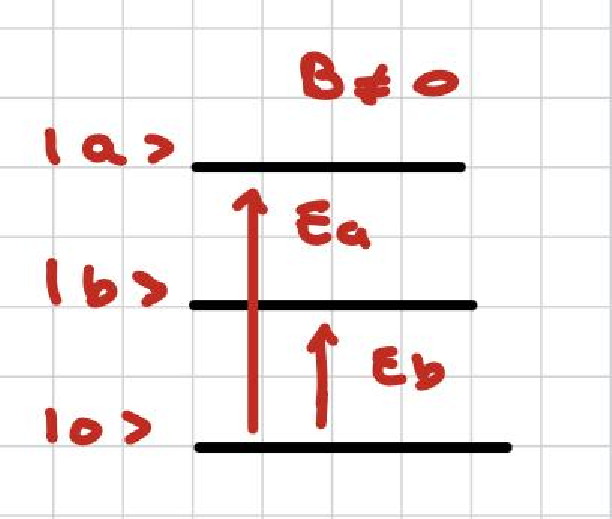
\includegraphics[width=0.4\textwidth]{images_in_pdf/3-/Grafico_18.pdf} 
\end{figure}
\end{comment}

When the luminescence emitted by the sample is measured, the circularly polarized components of the signal reflect this spin dynamics. 
For \textbf{zero magnetic field}, the emitted polarization typically shows a \textbf{monotonic decay}, as the non--equilibrium spin population relaxes toward thermal equilibrium with its characteristic \textbf{relaxation time}.
\begin{figure}[H]
    \centering
    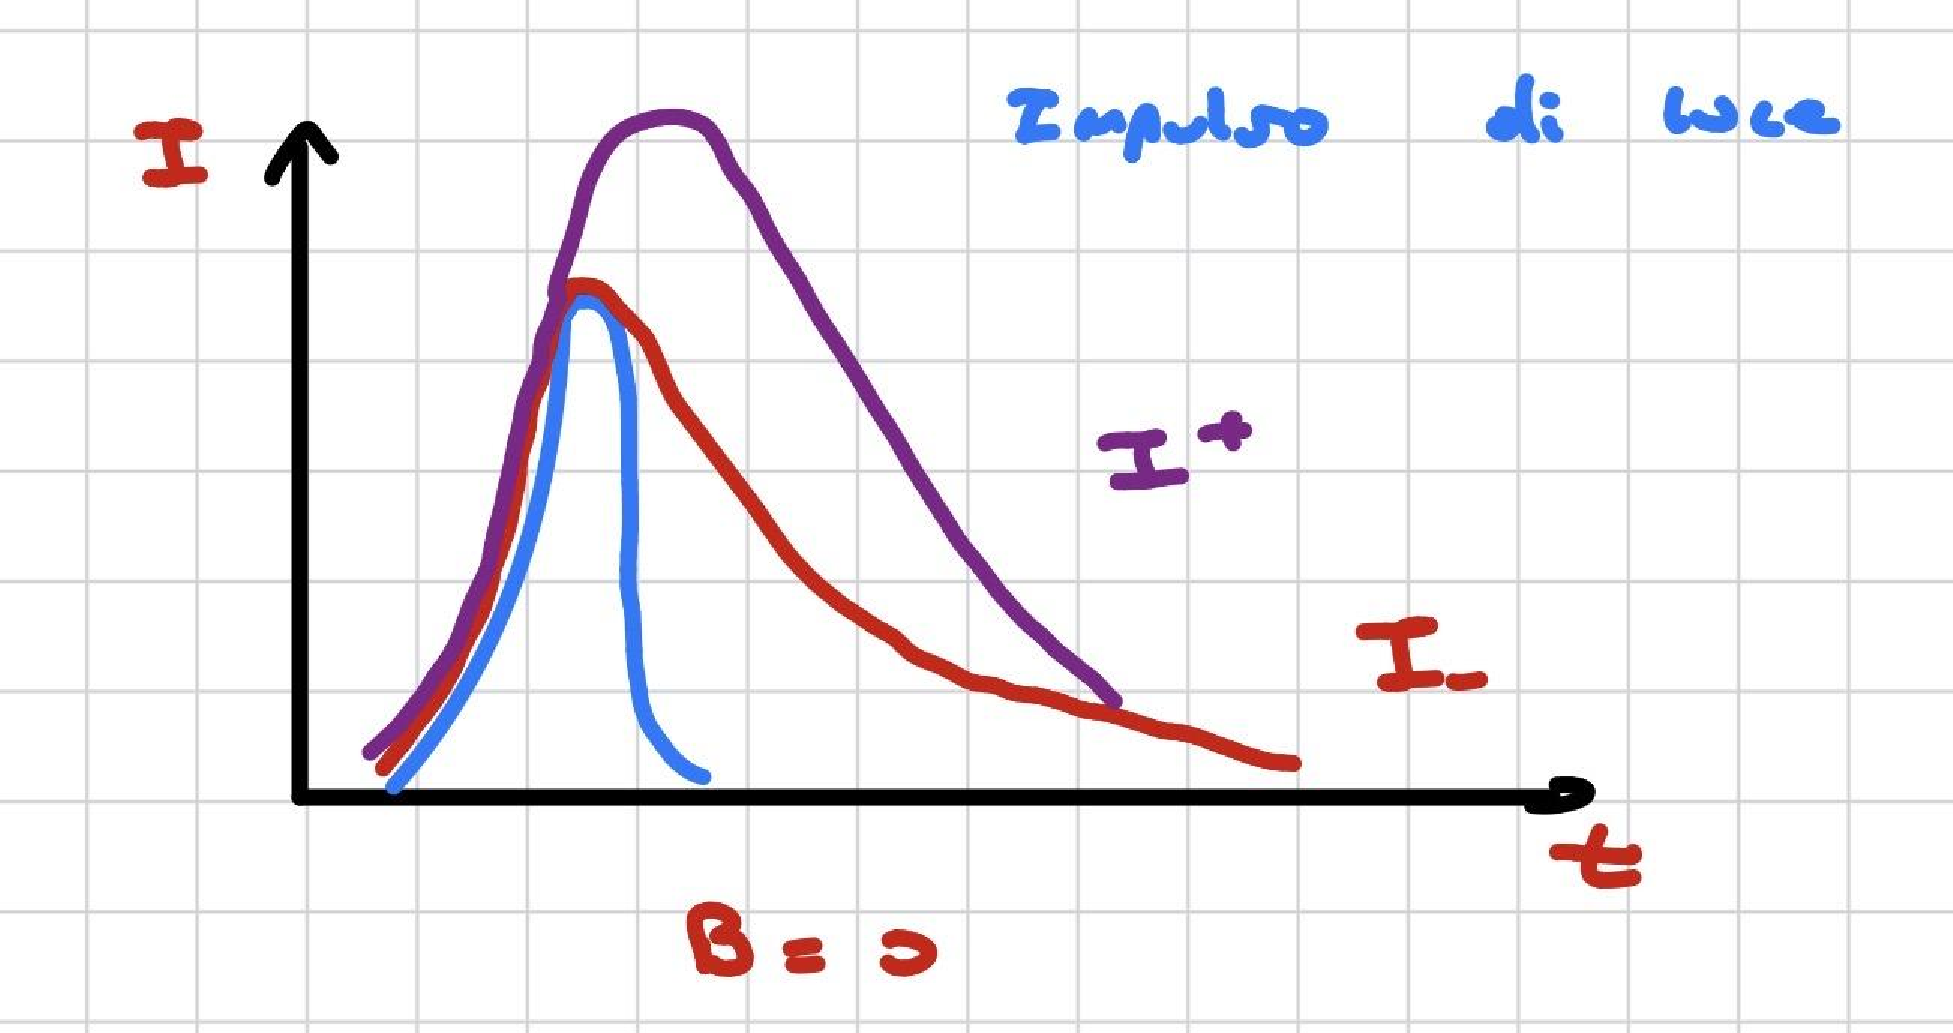
\includegraphics[width=0.6\linewidth]{images_in_pdf/3-/Grafico_19.pdf}
    \caption{$B=0$}
\end{figure}

In the figure, the blue curve represents the excitation pulse, while the other two curves correspond to the $\sigma^+$ and $\sigma^-$ components of the emitted luminescence. Their time dependence reflects an imbalance between the two circular polarizations, which gradually disappears because of spin relaxation.

\question{What happens when the magnetic field is turned on?}{Due to the Larmor precession, the two circular components now exhibit an oscillatory behavior, with alternating dominance in time.} 

\begin{figure}[H]
    \centering
    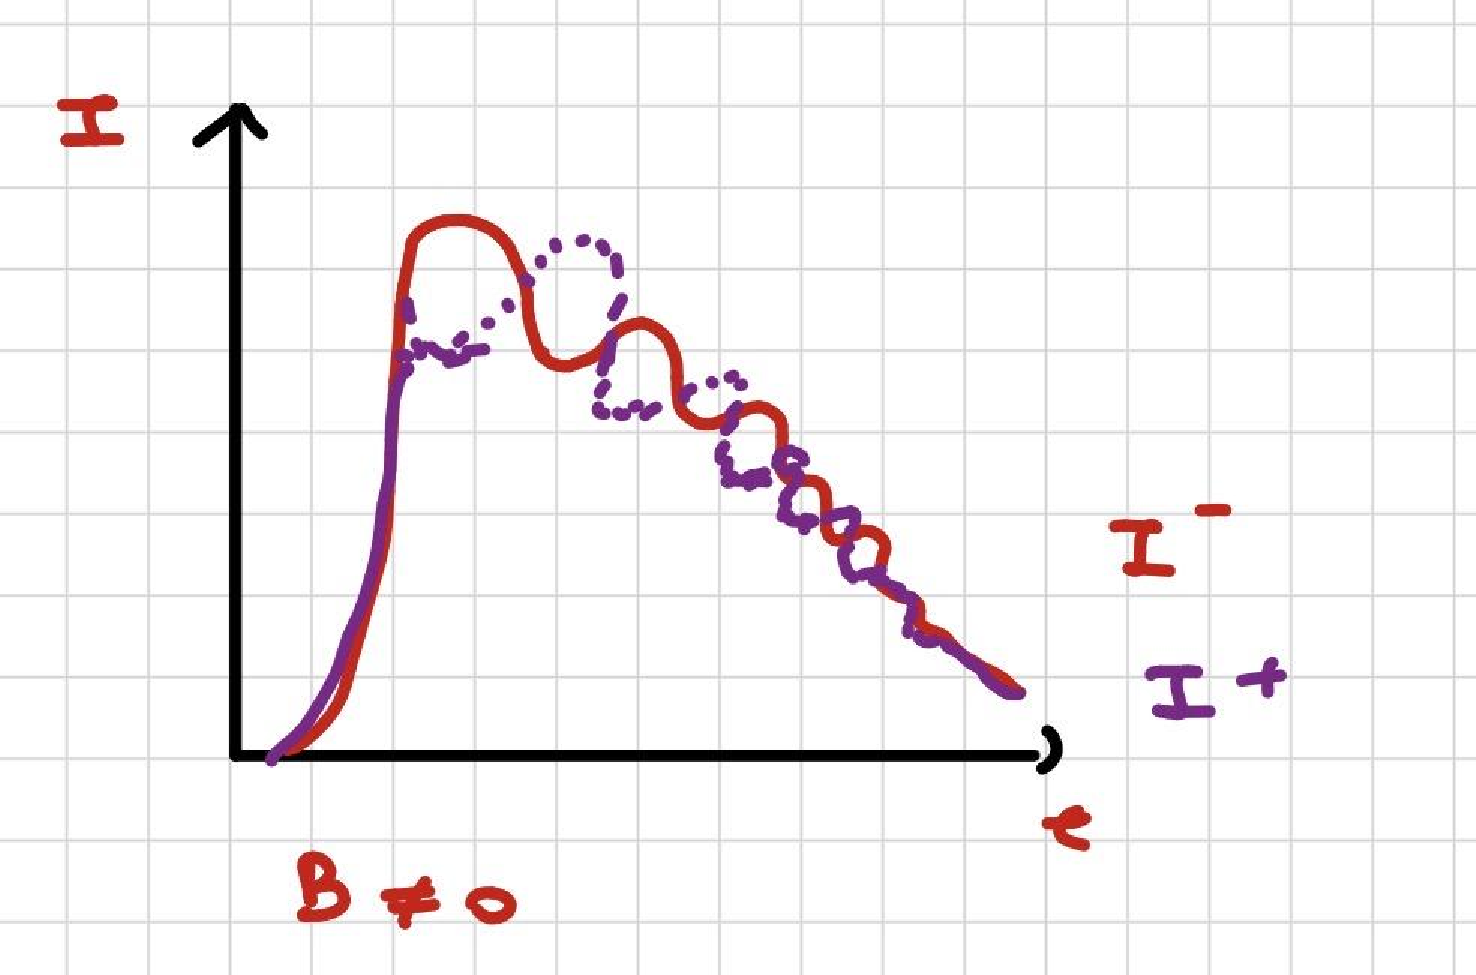
\includegraphics[width=0.6\linewidth]{images_in_pdf/3-/Grafico_20.pdf}
    \caption{$B \neq 0$}
\end{figure}

This relation is particularly useful since, measuring the oscillation frequency as a function of the magnetic field, one can \textbf{determine the $g$-factor} of the material. In the low-field regime, $\omega_L$ depends linearly on $B$, as expected from the Zeeman hamiltonian (Eqn.~\ref{eqn:3-zeeman-hamiltonian}).

At sufficiently high magnetic fields, deviations from linear behavior may appear because of additional contributions such as band non-parabolicity, orbital effects, anisotropy of the $g$-factor, or mixing with other states. These effects are not essential for the basic picture, but they can become relevant in precise experiments.